\documentclass[12pt, a4paper, twoside]{article}

\usepackage[top=2.4cm, bottom=2.4cm, left=1.9cm, right=1.9cm]{geometry}
\usepackage[utf8]		%	Kódování zdrojových souborů je v UTF-8
	{inputenc}					% Balíček pro nastavení kódování zdrojových souborů

\usepackage{graphicx} % Balíček 'graphicx' pro vkládání obrázků
											% Nutné pro vložení log školy a fakultyd
\title{Vírový autofokusační modul pro holografický mikroskop}

\date{Brno 2019}

\usepackage{pdfpages}

\usepackage{xcolor}

\usepackage{multicol}

\definecolor{vecblue}{RGB}{0, 51, 153}
\definecolor{vecgreen}{RGB}{0, 100, 0}

%\setlength{\parlength}{1.2}
\linespread{1.1}
\author{Jakub Dokulil}

\usepackage{booktabs}

\usepackage{svg}

\usepackage{hyperref}

\usepackage[
	%nohyperlinks				% Nebudou tvořeny hypertextové odkazy do~seznamu zkratek
]{acronym}

\usepackage{pdfpages} % Balíček umožňující vkládat stránky z~PDF souborů


\usepackage{cmap} 		% Balíček cmap zajišťuje, že PDF vytvořené `pdflatexem' je
											% plně "prohledávatelné" a "kopírovatelné"

\usepackage{upgreek}	% Balíček pro sazbu stojatých řeckých písmem

\usepackage{amsmath}
\usepackage{amsfonts}

\usepackage{subcaption}

\usepackage[czech]    				
  {babel}     
\title{Přihláška do soutěže Česká hlavička}
\author{Jakub Dokulil}
\begin{document}

\includepdf[pages=1,pagecommand={}]{J_Dokulil_prihlaska-2019.pdf}
\includepdf[pages=2,pagecommand={}]{J_Dokulil_prihlaska-2019.pdf}

\section*{Abstrakt}

Koherencí řízený holografický mikroskop je zařízení, které kromě pozorování buněk umožňuje
také jejich kvantitativní analýzu. Avšak pro získání kvalitních dat je zapotřebí, aby byl mikroskop
správně nastavený, což mimo jiné závisí na defokusaci vzorku. Tento problém je v současnosti
řešen softwarovým autofokusem, který se pro některé aplikace jeví jako méně vhodný. Proto
byl navržen přídavný autofokusační modul, využívající metodu axiální lokalizace pomocí
výrových svazků. Optická sestava byla počítačově simulována a optimalizována v programu Zemax. Pro sestavu
byla navržena vhodná spirální maska. Na základě simulací byla sestavena experimentální
sestava, která byla otestována.

\section*{Synopse}

\subsection*{Úvod}

Koherencí řízený holografický mikroskop je zařízení umožňující ne jen pozorování buněk,
nýbrž také jejich kvantitativní analýzu, například získat data o rozložení suché hmoty v buňce.
Avšak pro získání dat je klíčové správné naladění mikroskopu. Jednou z~veličin na které naladění
závisí je defokusace vzorku. Mikroskop sice je vybaven softwarovým autofokusem, ten se
však pro některé aplikace jeví jako méně vhodný. Proto je zapotřebí navrhnout hardwarový
autofokusační systém, který bude detekovat axiální polohu vzorku. K čemuž je zapotřebí
použít vhodnou metodu axiální lokalizace.
Pro detekci axiální polohy se jeví jako vhodné použit metodu axiální lokalizace pomocí
vírových svazků. Interferencí dvou vhodně vybraných vírových svazků vzniká dvoulaloč\-na\-tá
rozptylová funkce bodu, která rotuje při defokusaci vzorku. z~její rotace tedy lze získat
informaci o velikost a směru defokusace.

\subsection*{Koherencí řízený holografický mikroskop}

Běžné metody používané v mikroskopii umožňují pouze kontrastní pozorování buněk a nedokáží
získávat kvantitativní data o buňkách (např. rozložení hmotnosti). Tato data lze získat
pomocí kvantitativního fázového zobrazování. Příkladem takové techniky je digitální holografická mi\-kro\-sko\-pi\-e.

Koherencí řízený holografický mikroskop (CCHM -- Coherence Controlled Holographic Mi\-cro\-scope), jehož schéma lze vidět na obrázku \ref{fig:CCHM_schema} \cite{CCHM}, je v principu interferometrem. Světlo z~ne\-ko\-he\-rent\-ní\-ho zdroje S je rozděleno do~referenční a předmětové větve. Svazky z~jednotlivých větví se skládají ve výstupní rovině OP, kde tvoří hologram. Jeho následnou rekonstrukcí lze získat fázový obrázek jako je například obrázek \ref{fig:bunky} \cite{bunky2016}.

\begin{figure}
  \centering
  \includegraphics[width=0.6\textwidth]{obrazky/teor/CCHM.jpeg}
  \caption{Schéma koherencí řízeného holografického mikroskopu. Zdroj světla (S),
  kolektor (L), děliče svazku (BS), zrcádka (M), kondenzory (C), rovina vzorku (Sp), referenční
  rovina (R), mikroskopové objektivy (O), tubusové čočky (TL), difrakční mřížka (DG),
  výstupní čočka (OL), výstupní rovina (OP), detektor (D). $\alpha$ je difrakční úhel prvého řádu difrakční mřížky DG. Převzato a upraveno z~\cite{CCHM}. }
  \label{fig:CCHM_schema}
\end{figure}

\begin{figure}[h!]
  \includegraphics[width=\textwidth]{obrazky/teor/bunky.png}
  \caption[Fázový obrázek buněk.]{Fázové obrázky LW13K2 pořízené mikroskopem TESCAN Q-PHASE. Převzato z~\cite{bunky2016}.}
  \label{fig:bunky}
\end{figure}

Pro naladění mikroskopu je klíčová veličina holografický signál $w$ \cite{zbynek_disertace}. Ten závisí na 3 veličinách: rozdílu optických drah mezi větvemi $\Delta L$, vektoru posuvu obrazových polí $\vec{q_f}$ a defokusaci $\Delta z$. Graf závislosti signálu $w$ na defokusaci $\Delta z$ lze vidět na obrázku \ref{fig:defocus} \cite{zbynek_disertace}. Velikost ho\-lo\-gra\-fi\-cké\-ho signálu $w$ klesá při drobné změně kterékoli ze tří veličin. Proto je mikroskop vybaven justážními procedurami, které jej před prováděním experimentu naladí a během experimentu jej udržují najustovaný. Systém, starajíce se, aby mikroskop zůstal zafokusován je pouze softwarový, což se pro některé aplikace (například pozorování mitózy) jeví jako méně vhodné, proto je zapotřebí vybavit mikroskop hardwarovým autofokusem.

\begin{figure}[t!]
  \centering
  \includegraphics[width=0.4\textwidth]{obrazky/teor/d_z.pdf}
  \caption{Závislost holografického signálu $\bar{w}$ na defokusaci $\Delta z$ objektivu O$_1$. Převzato z~\cite{zbynek_disertace}.}
  \label{fig:defocus}
\end{figure}

\subsection*{Optické víry}

% Obvyklými pojmy, se kterými pracujeme při popisu vln libovolného původu, jsou amplituda a fáze. Ačkoliv je fáze při popisu elektromagnetických vln pomocnou veličinou, zavedení vlnoplochy, definované jako plochy konstantní fáze, poskytuje názornou představu o šíření a transformaci elektromagnetického záření. 
V běžných případech je vlnoplocha světla popsána spojitou funkcí. V rámci standardních metod popisu elektromagnetického záření byly ne\-spo\-ji\-to\-sti vlnoplochy považovány za oblasti, ve~kterých popis selhává, a nebyl na ně brán zřetel. Nová oblast moderní fyzikální optiky, nazývaná singulární optika, pracuje se širokou škálou jevů souvisejících~s fázovými singularitami optických polí a~s~jejich fázovou topologií \cite{bouchal2003}. Tedy s~optickými víry. Vír v optickém slova smyslu je typem fázové ne\-spo\-ji\-tost\-i, ve kterém má vlnoplocha tvar šroubovice postupující okolo nespojitého centra na optické ose. Pro každý vír je rozhodující veličinou topologický náboj. Ten udává kolik listů vlnoplocha má, jeho znaménko pak určuje směr rotace. Topologický náboj víru je ilustrován na obrázku~\ref{fig:top_naboj}~\cite{olomouc-viry}.



\begin{figure}[h!]
  \centering
  \includegraphics[width=0.25\textwidth]{obrazky/teor/topologicky_naboj_ch.pdf}
  \caption[Ilustrace vírového svazku.]{Na obrázku jsou zobrazeny tvary vlnoploch pro víry s různým topologickým nábojem $l$, fázové masky, kterými jsou tvořeny, a rozptylové funkce bodů (PSF -- \emph{Point Spread Function}) vzniklých fokusací daného svazku. Převzato a upraveno z~\cite{olomouc-viry}.}
  \label{fig:top_naboj}
\end{figure}

Velmi slibnou aplikací optických vírů je jejich použití na lokalizaci osové polohy. Nejčastěji je toho využito v mikroskopech pro získání 3D informace. Mikroskop je doplněn o 4$f$ systém s~prostorovým modulátorem světla v aperturní rovině mikroskopu, který vytváří dva optické víry. Ty spolu interferují a vytváří dvoučetnou rozptylovou funkci bodu (DH PSF -- \emph{double helix point spread function}). Tato funkce má podobu dvoučetné symetrie, která se projevuje jako dvě světlé stopy (laloky). Při praktickém použití metody je sledováno rozostření jasného bodu vzorku v předmětovém prostoru objektivu mikroskopu, které se projevuje rotací DH PSF v rovině kamery. Při pevné pozici detektoru je možné z~úhlového otočení DH PSF stanovit axiální pozici zobrazeného bodu s nanometrovou přesností \cite{Bouchal2015}.

\begin{figure}[h]
  \centering
  \includegraphics[width=\textwidth]{obrazky/teor/umisteni_maska_ch.pdf}
  \caption[Sestava pro axiální lokalizaci.]{Sestava pro axiální lokalizaci. O je mikroskopový objektiv, TL je tubusová čočka, $f$ jsou jejich ohniska, $\pm\Delta z$ je defokusace obrazového bodu, $ \Delta\beta_m$ je rozdíl propagačních konstant dvou vln, SM je spirální maska. Převzato a upraveno z~\cite{oe-2015}.}
  \label{fig:ax_loc_setup}
\end{figure}

Při užití spirální masky pro vytvoření optických vírů, je zapotřebí umístit masku do~aperturní roviny mikroskopového objektivu O, jak lze například vidět na obrázku \ref{fig:ax_loc_setup} \cite{oe-2015}.

\subsection*{Návrh autofokusačního modulu}

Cílem je sestrojit zařízení, umožňující axiální lokalizaci pomocí vírových svazků. Použití této metody je vhodné právě proto, že z~natočení DH PSF lze zjistit informaci o velikosti a směru defokusace. Sestavu lze lze rozdělit na dvě části:
\begin{description}
  \item[Osvětlovací část] do~systému dodává IR záření, který modul využívá a které CCHM jej nevyužívá pro zobrazování.
  \item[Zobrazovací část] slouží k zobrazení bodu vzorku, tak aby bylo dosaženo samozobrazení a~vznikla DH PSF.
\end{description}

\begin{figure}
  \centering
  \includegraphics[height=0.80\textheight]{obrazky/konstrukce/setup-sazba_ch}
  \caption[Schéma modulu]{
Schéma modulu.    
%Infračervené záření z~LED je mikroskopovým objektivem zobrazeno do~5$\upmu$m dírkové clony. Ta slouží jako pseudobodový zdroj světla. Best form čočka vytváří kolimovaný svazek, který je objektivem zobrazen na sklíčko, od kterého se odráží zpět do~objektivu. Za ním je IR záření odděleno od zbytku světla pomocí dichronického zrcátka. Děličem svazku je pak odveden do~zobrazovací části. V té je umístěn $4f$ systém se spirální maskou, která vytváří dva optické víry. Spirální maska je zároveň umístěna v ohniskové rovině tubusové čočky a na kameře vzniká DH PSF. Celá soustava využívá infračerveném záření o vlnové délce $850\,\mathrm{nm}$.
}
  \label{fig:setup}
\end{figure}

Teoretické schéma modulu lze vidět na obrázku \ref{fig:setup}. Světlo z~IR LED je kolektorem zaostřeno do~dírkové clony, jejíž průměr $d$ byl vypočítán tak, aby se podle Rayleighova kritéria clona zobrazila do~roviny vzorku jako difrakčně limitovaný jasný bod:
$$ d=\frac{ 0,\!61\cdot z~\cdot \lambda}{N\!A} = \frac{ 0,\!61\cdot 5 \cdot 0,850\,\upmu\mathrm{m}}{0,\!5} \approx 5\, \upmu \mathrm{m}, $$
kde $N\!A$ je numerická apertura mikroskopového objektivu Plan Fluor 20, $Z$ je absolutní hodnota příčného zvětšení mikroskopového objektivu a kolimátoru a $\lambda$ je vlnová délka užitého světla. 

Svazek vcházející z LED je zkolimován best form čočkou s ohniskovou vzdáleností $f_k=50 \,\mathrm{mm}$, jelikož best form čočky jsou nejméně zatíženy sférickou vadou při zobrazování z~bodu do~nekonečna. Následně je svazek zfokusován mikroskopovým objektivem na vzorek, kde vytváří difrakčně limitovaný obraz clony. 

Záření se od vzorku odráží a je odkloněno do~zobrazovací části. Jelikož maska nemůže být umístěna do~zadní ohniskové roviny objektivu (mikroskop by nešel používat), tak se v zobrazovací části nachází 4$f$ systém zobrazující tuto rovinu do~roviny spirální masky. Spirální maska vytváří dva víry, které jsou fokusovány tubusovou čočkou na kameru.

Jednotlivé části modulu byly počítačové simulovány a optimalizovány v programu Zemax. Schémata s vytrasovanými paprsky lze vidět na obrázcích \ref{fig:osv_zem} a \ref{fig:zobr_zem}. Na obrázku \ref{fig:spot_20} se nachází stopa bodu zobrazeného zobrazovací částí soustavy. Tyto simulace nezahrnovaly spirální masku, jelikož Zemax je program pro geometrickou nikoli vlnovou optiku.

Spirální maska byla navržena a simulována Ing. Petrem Bouchalem, Ph.D. pro dosažení optimální přesnosti detekce rozostření při užití objektivů se zvětšením 10$\times$, 20$\times$ a případně i~40$\times$. Teoretické hodnoty přesností detekce lze vidět v tabulce~\ref{tab:presnost}. Maska obsahuje dvě soustředná mezikruží, každé rozdělené do~osmi segmentů postupně posouvajících fázi v rozsahu fáze 2$\uppi$. Zóny vytváří dva víry s topologickými náboji $l_1=-1$ a $l_2=+1$. Maska byla následně realizována Ing. Jakubem Sadílkem v laboratořích CEITECu NANO.

\begin{figure}[t]
  \centering
  \includegraphics[width=0.90\textwidth]{obrazky/konstrukce/osvetleni_zem_ch.pdf}
  \caption[Schéma a simulace chodu paprsků osvětlovací částí.]{Nalevo je teoretické schéma osvětlovací části modulu. Napravo je simulace chodu paprsků provedená programem Zemax.}
  \label{fig:osv_zem}
\end{figure}

\begin{figure}[t]
  \centering
  \includegraphics[angle=90, height=0.65\textheight]{obrazky/konstrukce/zobrazeni_ch.pdf}
  \caption[Schéma a simulace chodu paprsků osvětlovací částí.]{Nalevo je teoretické schéma zobrazovací části modulu. Napravo je simulace chodu paprsků provedená programem Zemax.}
  \label{fig:zobr_zem}
\end{figure}

\begin{figure}[t]\centering
  \includegraphics[width=0.28\textwidth]{obrazky/konstrukce/spot_20.pdf}
  \caption[Stopa bodu zobrazeného zobrazovací částí soustavy.]{Stopa bodu zobrazeného zobrazovací částí soustavy s objektivem Plan Fluor 20. Modré jsou jednotlivé vytrasované paprsky. Černá kružnice je velikost difrakčně limitované stopy bodu s poloměrem 18 $\upmu$m. }
  \label{fig:spot_20}
\end{figure}

\begin{figure}[t]
  \centering
  \includegraphics[width=0.55\textwidth]{obrazky/konstrukce/vykres_SM}
  \caption{Výkres navržené masky s očíslováním jednotlichých segmentů $j$.}
  \label{fig:vykres_masky}
\end{figure}


\begin{table}[]
  \caption{Teoretické hodnoty přesnosti detekce defokusace $\Delta z$ pro jednotlivé objektivy.}
  \centering
  \begin{tabular}{lp{2.7cm}p{2.7cm}p{2.7cm}}
    \toprule
    Objektiv& Hloubka ostrosti $[\upmu\mathrm{m}]$& Přesnost lokalizace $[\mathrm{nm}]$& Rozsah detekce $[\upmu\mathrm{m}]$\\
    \midrule
    Plan 10&13,6& 1 000 &193\\
    Plan Fluor 20&3,4&270&48\\
    Plan Fluor 40&0,94&70&12\\
    Plan Apo 40&1,51&70&12\\
    \bottomrule\\
  \end{tabular}
  \label{tab:presnost}
\end{table}
\cleardoublepage

\subsection*{Realizace experimentu}
Podle návrhu modulu byla poskládána experimentální sestava. Při realizaci byl pro mechanické uložení jednotlivých komponent použit cage systém od firmy Thorlabs. Při stavbě experimentálního modulu nebylo použito dichronické zrcadlo, jelikož sestava zatím není napojena na CCHM, tudíž není zapotřebí dělit IR záření od viditelného světla. Místo vzorku bylo do~soustavy umístěno zrcátko na mikrometrickém posuvu, které jej simulovalo.

\begin{figure}[t]
  \centering
  \includegraphics[width=0.8\textwidth]{obrazky/experiment/foto_s_popisky.pdf}
  \caption{Experimentální sestava.}
  \label{fig:exp_setup}
\end{figure}

Systém byl postupně, komponent po komponentu sestaven a najustován. Poloha jednotlivých komponent byla nejdříve přibližně odměřena posuvným měřidlem a následně doupravena.

Následně byla získána DH PSF rotující při defokusaci vzorku. Na obrázku \ref{fig:vysl_20} lze vidět DH PSF zachycené při použití objektivu Plan Fluor 20. Výsledky pro jednotlivé objektivy vynesené do~grafu lze vidět na obrázku \ref{fig:rotace_grafy}.

\begin{figure}[h!] \centering
  \begin{subfigure}{0.30\textwidth}
    \includegraphics[width=\textwidth]{obrazky/20_se_streditkem/4.png}
    \caption{}
  \end{subfigure}
  \begin{subfigure}{0.30\textwidth}
    \includegraphics[width=\textwidth]{obrazky/20_se_streditkem/6.png}
    \caption{}
  \end{subfigure}
  \begin{subfigure}{0.30\textwidth}
    \includegraphics[width=\textwidth]{obrazky/20_se_streditkem/8.png}
    \caption{}
  \end{subfigure}

  \begin{subfigure}{0.30\textwidth}
    \includegraphics[width=\textwidth]{obrazky/20_se_streditkem/10.png}
    \caption{}
  \end{subfigure}
  \begin{subfigure}{0.30\textwidth}
    \includegraphics[width=\textwidth]{obrazky/20_se_streditkem/12.png}
    \caption{}
  \end{subfigure}
  \caption[Víry získané s objektivem Nikon plan 20.]{Zachycené DH PSF s objektivem Nikon Plan Fluor 20 mezi jednotlivými snímky (a) až (e) je nastaven rozdíl defokusace o 2 $\upmu$m. Výška obrázku odpovídá je 440 $\upmu$m.}
  \label{fig:vysl_20}
\end{figure}

\begin{figure}[h!] \centering
  \begin{subfigure}{0.6\textwidth}
    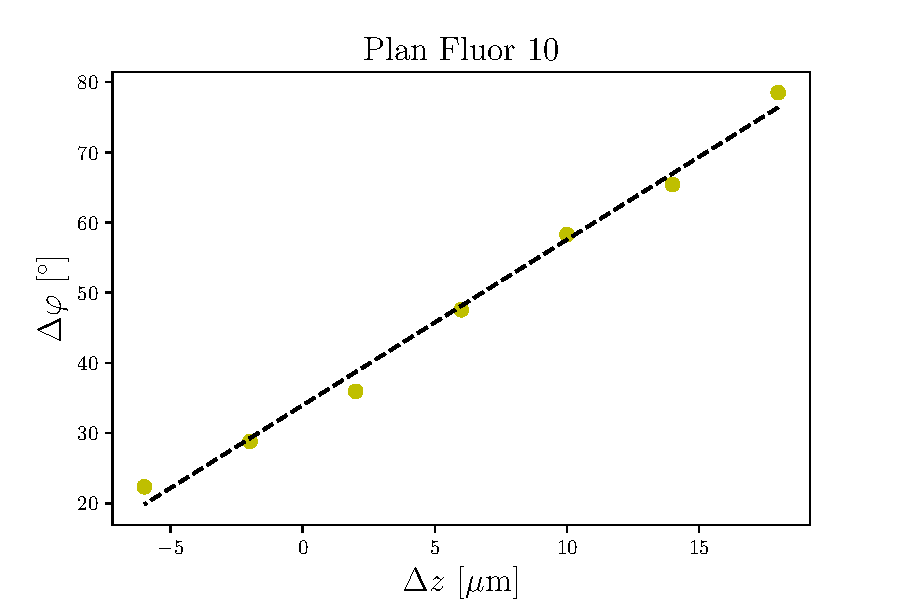
\includegraphics[width=\textwidth]{obrazky/experiment/vysledek_10}
    \caption{}
  \end{subfigure}
  \begin{subfigure}{0.6\textwidth}
    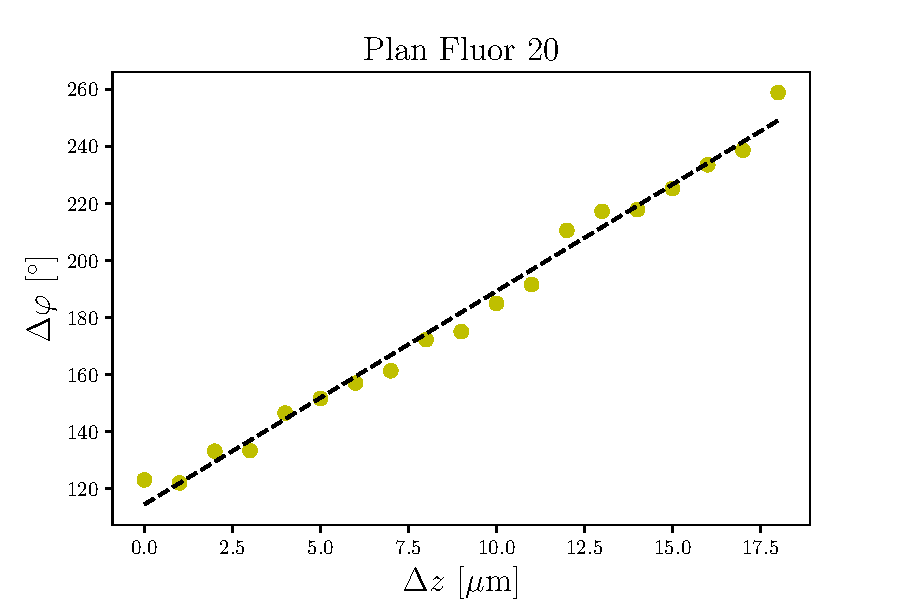
\includegraphics[width=\textwidth]{obrazky/experiment/vysledek_20}
    \caption{}
  \end{subfigure}
  \caption{Graf závislosti rotace DH PSF $\Delta\varphi$ na defokusaci objektivu $\Delta z$, (a) při použití objektivu Plan Fluor 10, (b) při použití objektivu Plan Fluor 20. Měřená data (žluté body) jsou lineárně proloženy (přerušovaná přímka). }
  \label{fig:rotace_grafy}
\end{figure}

\subsection*{Závěr}

V důsledku je cílem vylepšit koherencí řízený holografický mikroskop tak, aby z~něj bylo možné získávat kvalitnější výstupy. Byl navržen hardwarový autofokusační modul pro tento mikroskop. Byl úspěšně počítačově simulován v programu Zemax. Následně byl modul ex\-pe\-ri\-men\-tál\-ně realizován. Navržená sestava byla sestavena a najustována. Byla navržena a vyrobena spirální maska pro tento systém. Správnost justáže byla ověřena zachycením DH PSF se spirální maskou. Byla zachycena DH PSF, rotující s defokusací vzorku. Jednotlivé laloky byly při užití správné dírkové clony rozeznatelné a správně rotovaly při defokusaci vzorku, viz obrázek \ref{fig:rotace_grafy}, což potvrzuje správnost optického návrhu a jeho použitelnost a přesnost detekce rozostření vzorku v CCHM mikroskopu.


\begin{thebibliography}{30}
  \bibitem{CCHM}LOŠŤÁK, M; CHMELÍK, R; SLABÁ, M; SLABÝ, T, 2014: Coherence-controlled holographic microscopy in diffuse media. OPTICS EXPRESS 22 (4), p. 4180 - 4195. DOI: \url{https://doi.org/10.1364/OE.22.004180}.

  \bibitem{bunky2016} ŠTRBKOVÁ, Lenka, Daniel ZÍCHA, Pavel VESELÝ a Radim CHMELÍK. Automated classification of cell morphology by coherence-controlled holographic microscopy. \textit{J. of Biomedical Optics}. 2017. DOI: \url{https://doi.org/10.1117/1.JBO.22.8.086008}.

  \bibitem{zbynek_disertace} DOSTÁL, Z. \emph{Automatizované procedury pro~Koherencí řízený holografický mikroskop.} Vysoké učení technické v~Brně, Fakulta strojního inženýrství, 2016, 82 s., Vedoucí prof.~RNDr.~Radim Chmelík,~Ph.D.

  \bibitem{bouchal2003}BOUCHAL, Zdeněk. Optické víry -- nový směr rozvoje singulární optiky. \emph{Čs. čas. fyz.} 2003, (1), 11-19.

  \bibitem{olomouc-viry}Světelné víry|Laboratoř. \textit{Laboratoř digitální optiky} [online]. Olomouc, 2015 [cit. 2018-09-29]. Dostupné z: \url{http://ldo.optol.cz/cs/?page_id=2711}

  \bibitem{bouchal_novy}BOUCHAL, Petr a Zdeněk BOUCHAL. Flexible non-diffractive vortex microscope for three-dimensional depth-enhanced super-localization of dielectric, metal and fluorescent nanoparticles. Journal of Optics. 2017, 19(10). DOI: \url{10.1088/2040-8986/aa87fb}. ISSN 2040-8978.

  \bibitem{Bouchal2015}BOUCHAL, Zdeněk a Petr BOUCHAL. Optické víry aneb jak roztočit světlo. \textit{Československý časopis pro fyziku}. 2015, 2015(5.), 351--354.

  \bibitem{olomouc-web}Prostorová lokalizace mikročástic|Laboratoř. \textit{Laboratoř digitální optiky} [online]. Olomouc, 2015 [cit. 2018-09-26]. Dostupné z: \url{http://ldo.optol.cz/cs/?page\_id=3021}

  \bibitem{bouchal2014}BOUCHAL, Petr a Zdeněk BOUCHAL. Non-iterative holographic axial localization using complex amplitude of diffraction-free vortices. \emph{Optics express}. 2014, 22(24), 30200 - 30216. DOI: \url{http://dx.doi.org/10.1364/OE.22.030200}.

  \bibitem{oe-2015}Baranek, M; Bouchal, P; Siler, M; Bouchal, Z, 2015: \textit{Aberration resistant axial localization using a self-imaging of vortices}. OPTICS EXPRESS 23(12), p. 15316 - 15331, DOI: \url{https://doi.org/10.1364/OE.23.015316}

\end{thebibliography}


\includepdf[pages=1,pagecommand={}]{J_Dokulil_doporuceni_Prof_Chmelik.pdf}
\end{document}